\documentclass[12pt]{cheatsheet}
\usepackage{blindtext}
\usepackage{enumitem}
\setlist{itemsep=0.2em, topsep=0.2em}
\usepackage{amsmath}
\usepackage{xcolor}
\usepackage{cancel}
\usepackage{tikz}
\usetikzlibrary{arrows.meta}


\author{Gian Maria Ernst - ernstg\\  \vspace*{0.2em} \vspace*{-0.2em}}\doctitle{Bioengineering}

\begin{document}
\small
\scalebox{0.7}{
\begin{tabular}{@{}lcc@{}}

Tera   & T      & $10^{12}$ \\
Giga   & G      & $10^{9}$ \\
Mega   & M      & $10^{6}$ \\
\end{tabular}
}
\scalebox{0.7}{
\begin{tabular}{@{}lcc@{}}
    Kilo   & k      & $10^{3}$ \\
    
    Milli  & m      & $10^{-3}$ \\
Mikro  & $\mu$  & $10^{-6}$ \\
\end{tabular}
}
\scalebox{0.7}{
\begin{tabular}{@{}lcc@{}}
Nano   & n      & $10^{-9}$ \\
Piko   & p      & $10^{-12}$ \\
Femto  & f      & $10^{-15}$ \\
\end{tabular}
}


\section*{Orientation of the cell}
Central Dogma of Molecular Biology
\[
\boxed{
    \begin{aligned}
        \text{DNA} \ &\xrightarrow{\text{transcription}} \text{mRNA} \xrightarrow{\text{translation}} \text{proteins}
    \end{aligned}
}
\]
Cells:\\
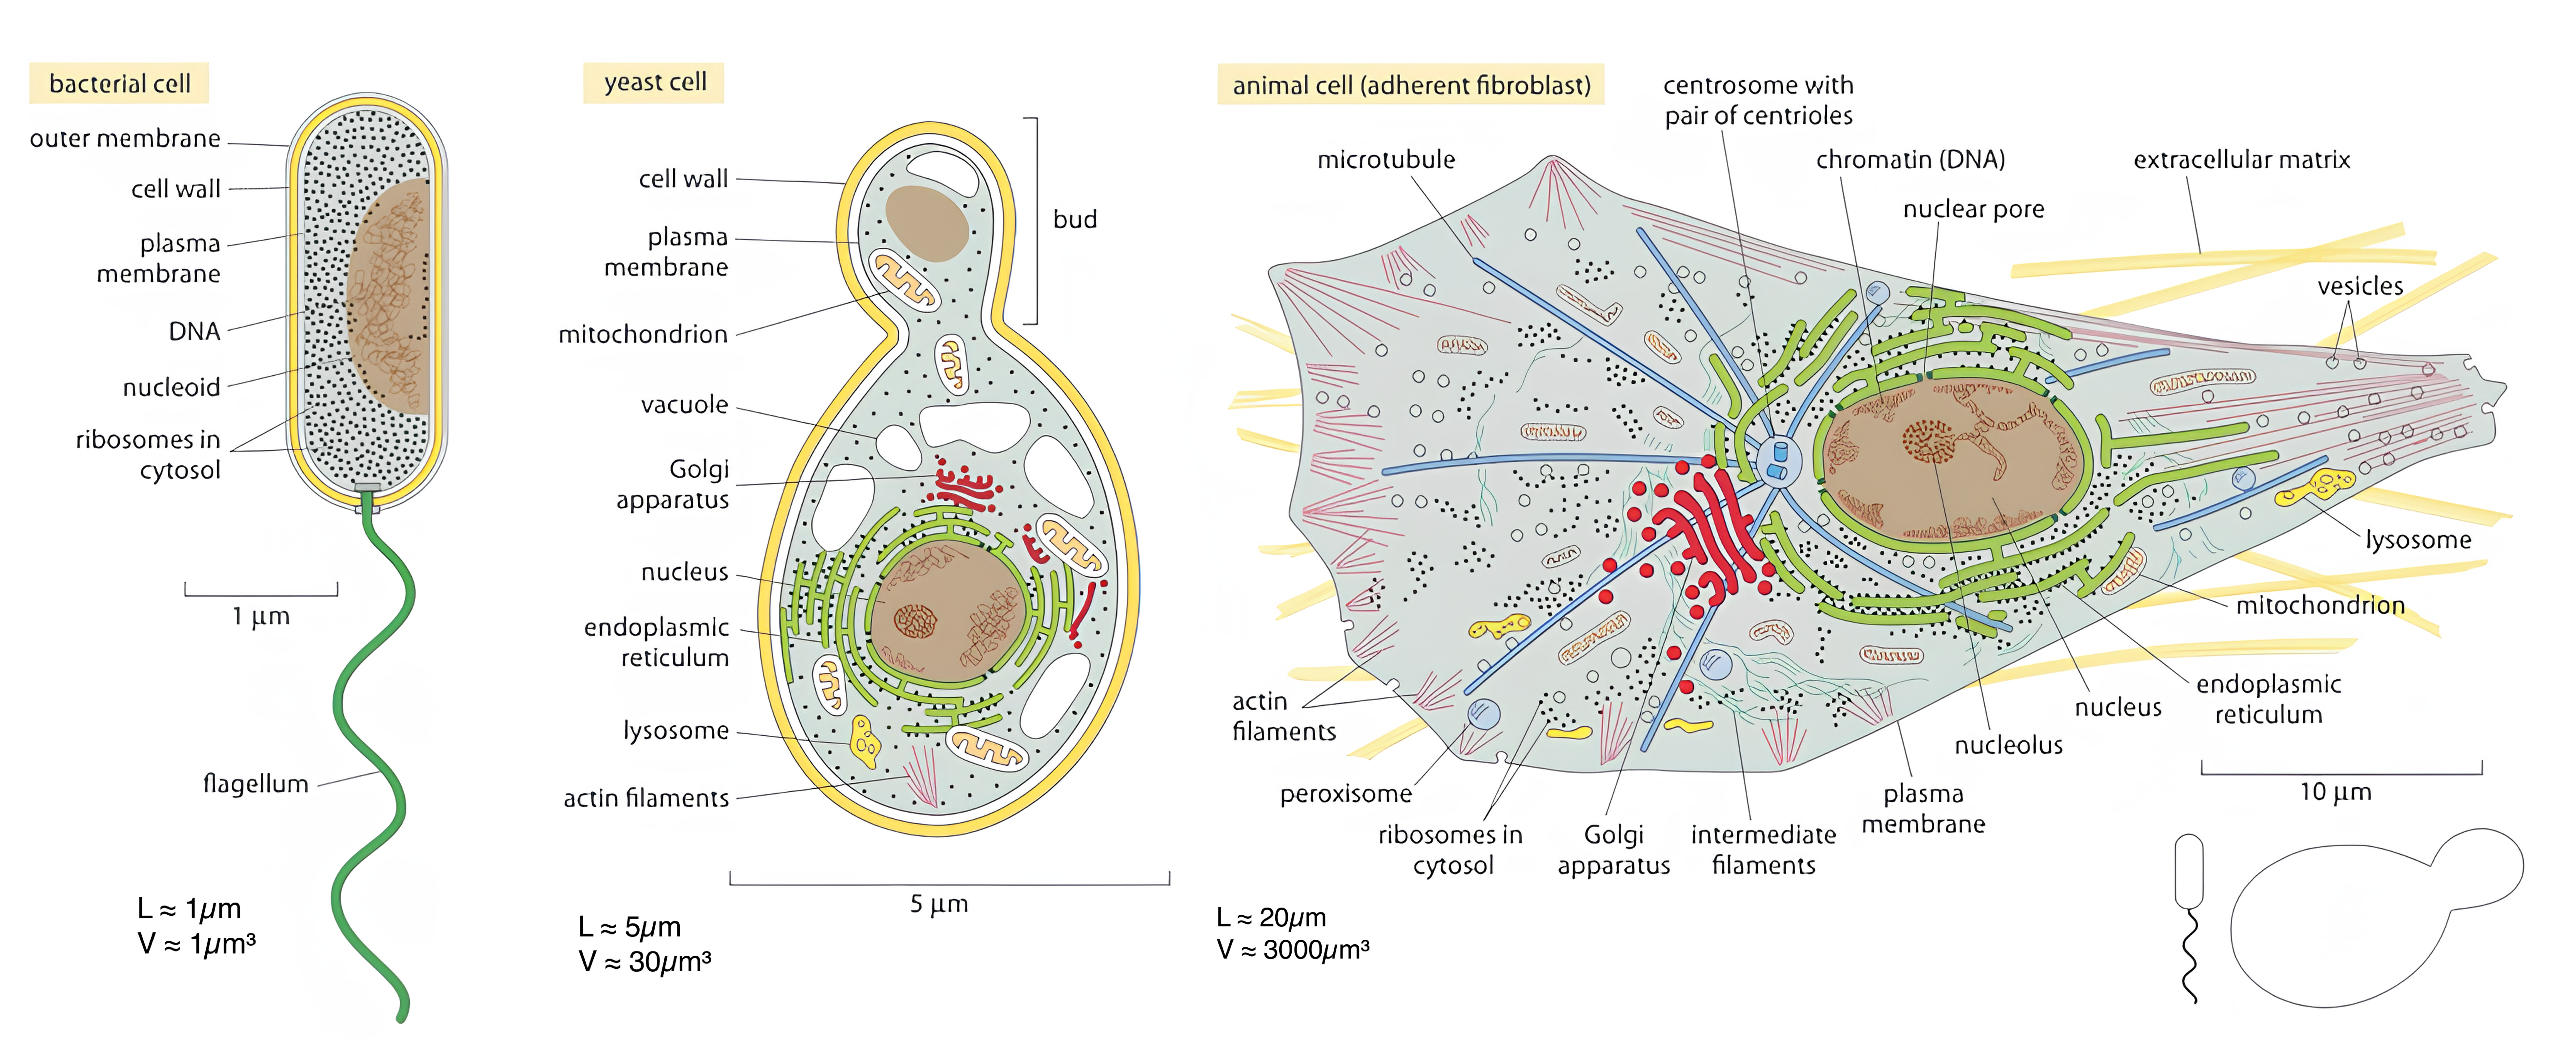
\includegraphics[width=7.3cm]{src/images/cell.png}

\begin{minipage}{0.45\linewidth}
    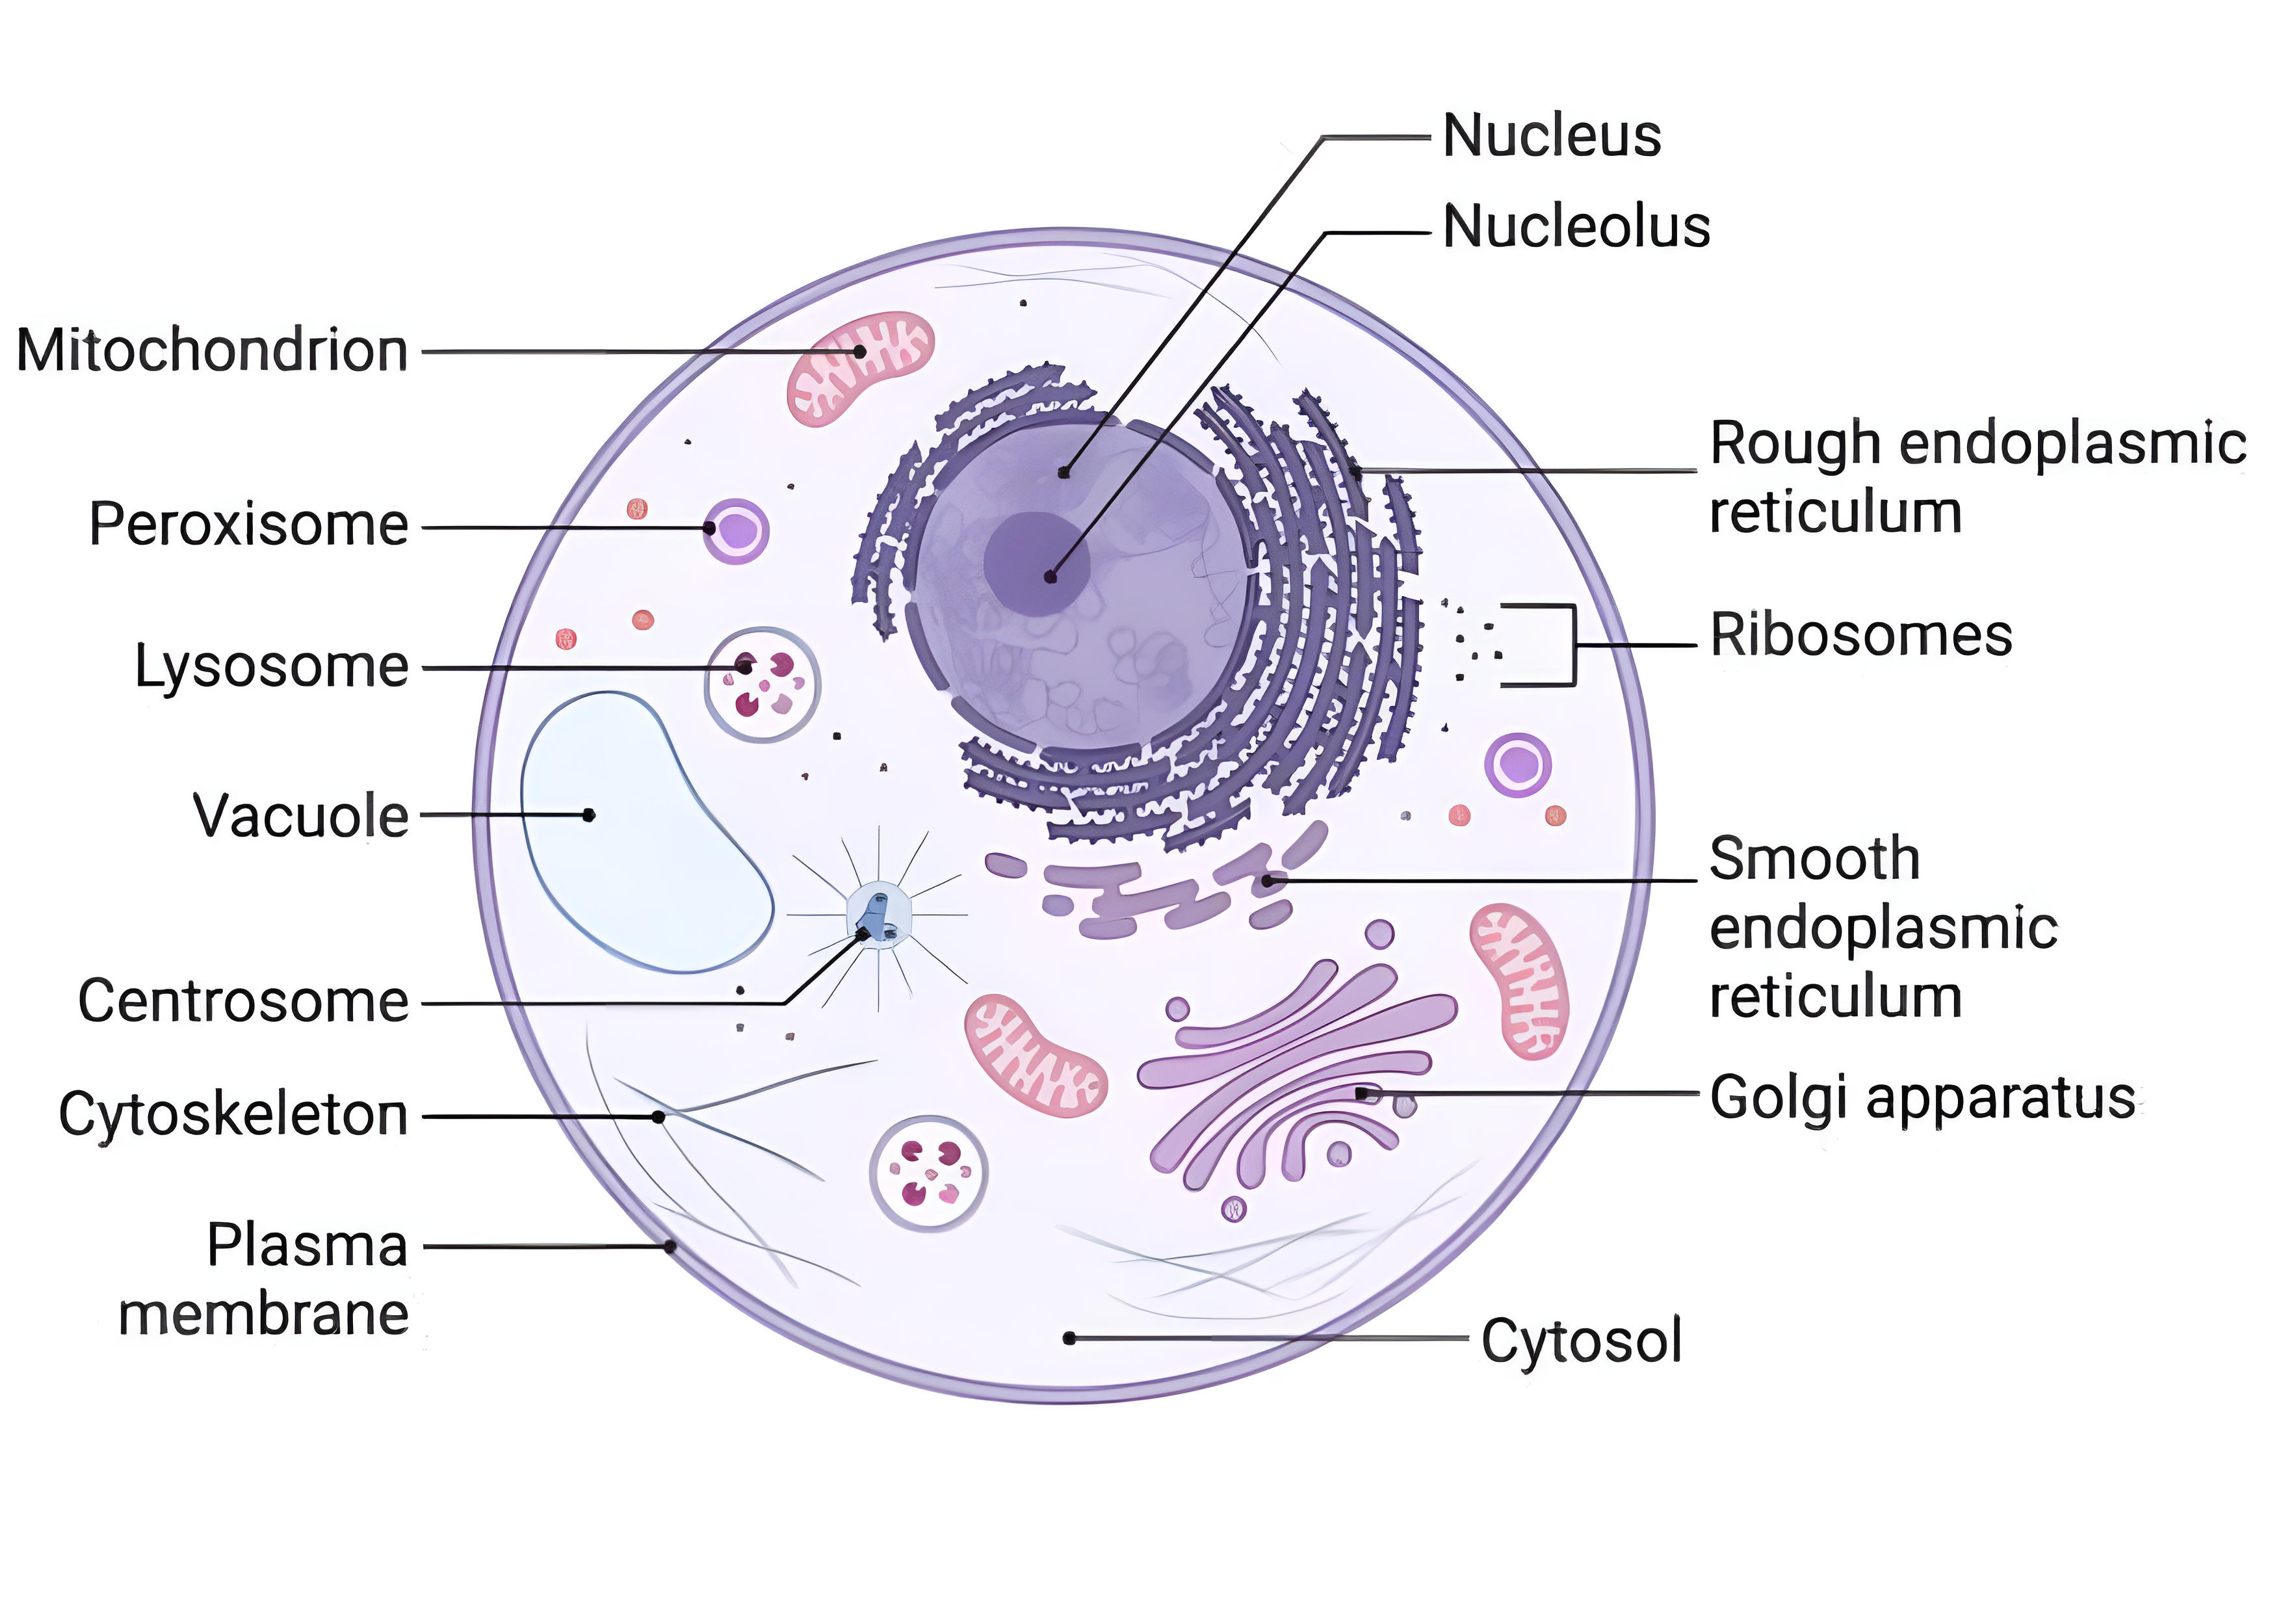
\includegraphics[width=3cm]{src/images/organelles.png}
\end{minipage}
\begin{minipage}{0.55\linewidth}
    \textbf{nucleus}: houses DNA for EK\\
    \textbf{nucleolus}: produces ribosomes/rRNA\\
    \textbf{mitochondria}: cellular respiration (prod. ATP)\\
    \textbf{ribosome}: produces proteins from mRNA transcripts\\
    
\end{minipage}
\vspace{1mm}
\textbf{RER, SER and Golgi}: involved in protein/lipid synthesis/processing\\
\textbf{cytoskeleton}: structure to cell, transport mol. in the cell or to enable the cell to move (cell migration)\\
\textbf{centrosome}: organizes microtubules during cell division allows the mother cell to split into 2 cells\\


\section*{Building Blocks}
\begin{minipage}{0.4\linewidth}
    Cell composition:\\
    \includegraphics[width=3cm]{src/images/cell_composition.png}
\end{minipage}
\begin{minipage}{0.45\linewidth}
    Main building blocks:\\
    \vspace{1mm}
    \includegraphics[width=4cm]{src/images/main_building_blocks.png}
\end{minipage}  

\begin{itemize}
\item \textbf{Lipids} (fatty acids): long-term energy storage, cell membrane structure, signaling molecules.
\item\textbf{Proteins} (amino acids): perform most of the cell's functions, including catalyzing reactions, signaling, and structural support.
\hspace{11mm} amino group $\textbf{NH}_2$, carboxyl group \textbf{COOH}
\item \textbf{Nucleic acids} (nucleotides): store and transmit genetic information (DNA, RNA), carry energy
\item \textbf{Carbohydrates} (Sugars): short-term energy storages and for structural support.
\end{itemize}
    

\subsection*{Enzymes (aka catalysts)}
\begin{itemize}
\item Accellerate reaction by lowering the activation energy
\item Are not consumed in the reaction
\item Are specific to the reaction they catalyze
\item Do not change the equilibrium point of the reaction.
\end{itemize}
\vfill \null \columnbreak

\subsection*{Bounds}
\begin{minipage}{0.5\linewidth}
    \[
    \boxed{        
            K_D = \frac{k_{off}}{k_{on}}
    }
    \]
\end{minipage}\begin{minipage}{0.4\linewidth}
\begin{align*}
    \text{Covalent} &\longleftrightarrow 100 k_B T\\
    \text{Ionic} &\longleftrightarrow 1-10 k_B T\\
    \text{Hydrogen} &\longleftrightarrow 1 k_B T\\
    \text{Van der Waals} &\longleftrightarrow 0.1 k_B T\\
    \text{Electrostatic} &\longleftrightarrow 0.1 k_B T
\end{align*}
\end{minipage} 

    $K_D$: Equilibrium constant\\
    indicates the ratio of free \& bound units\\
    $k_{off}$: Dissociation rate constant\\
    inverse of time protein dissociates from the ligand\\
    $k_{on}$: Association rate constant, speed of the reaction


\section*{Prozesse und Prozessketten}

\section*{Simulation}
¨
\section*{Urformen}

\section*{Pulvermetallurgie}

\section*{Umformen}

\section*{Trennen}

\section*{Fügen}





\end{document}